%%__________________________________________________________________||
\section{Results}
\label{sec:interpretation}

A likelihood model of the observations in all data samples is used to
obtain a consistent prediction of the SM backgrounds and to test for
the presence of a variety of signal models.  In each bin of \scalht
for events in the same category of \njet and \nb, the observation is
modelled as a Poisson-distributed variable around the sum of the SM
expectation and a potential signal contribution (assumed to be zero in
the following discussion). The SM expectation is related to the
expected yields in the \mj, \mmj, and \gj control samples via transfer
factors derived from simulation. Likelihood functions describe the
yields in the \scalht bins of the \mj, \mmj, and \gj control samples
in the same category of \njet and \nb as the signal region. The
systematic uncertainties summarised in Table~\ref{tab:bkgd_systs} are
accommodated in the likelihood function by nuisance parameters, the
measurements of which are assumed to follow a log-normal
distribution. In the presence of a non-zero signal contribution, the
CL$_{\mathrm{s}}$ technique~\cite{read, Cowan:2010js} is used to
determine upper limits on production cross section using asymptotic
formulae.

The expected number of events from SM processes is determined from a
simultaneous fit to the signal region and up to three control
samples. The likelihood function is maximised over all fit parameters
under the SM-only hypothesis.
Figures~\ref{fig:mono}--\ref{fig:sym}
summarise the observed yields and ``pre-fit'' and ``post-fit'' SM
expectations for signal candidate events in the monojet, asymmetric,
and symmetric categories, respectively. No significant tension is
observed between the predictions and data in the signal region, which
is well described by the SM-only hypothesis.

Figure~\ref{fig:mht-templates} shows distributions of observed counts
in data and also expected counts from SM background processes, as a
function of the \mht variable for two \nb categories at high \njet and
\scalht. %, which are expected to provide sensitivity to models with
%TeV-scale gluinos. 

\begin{figure}[!h]
  \begin{center}
    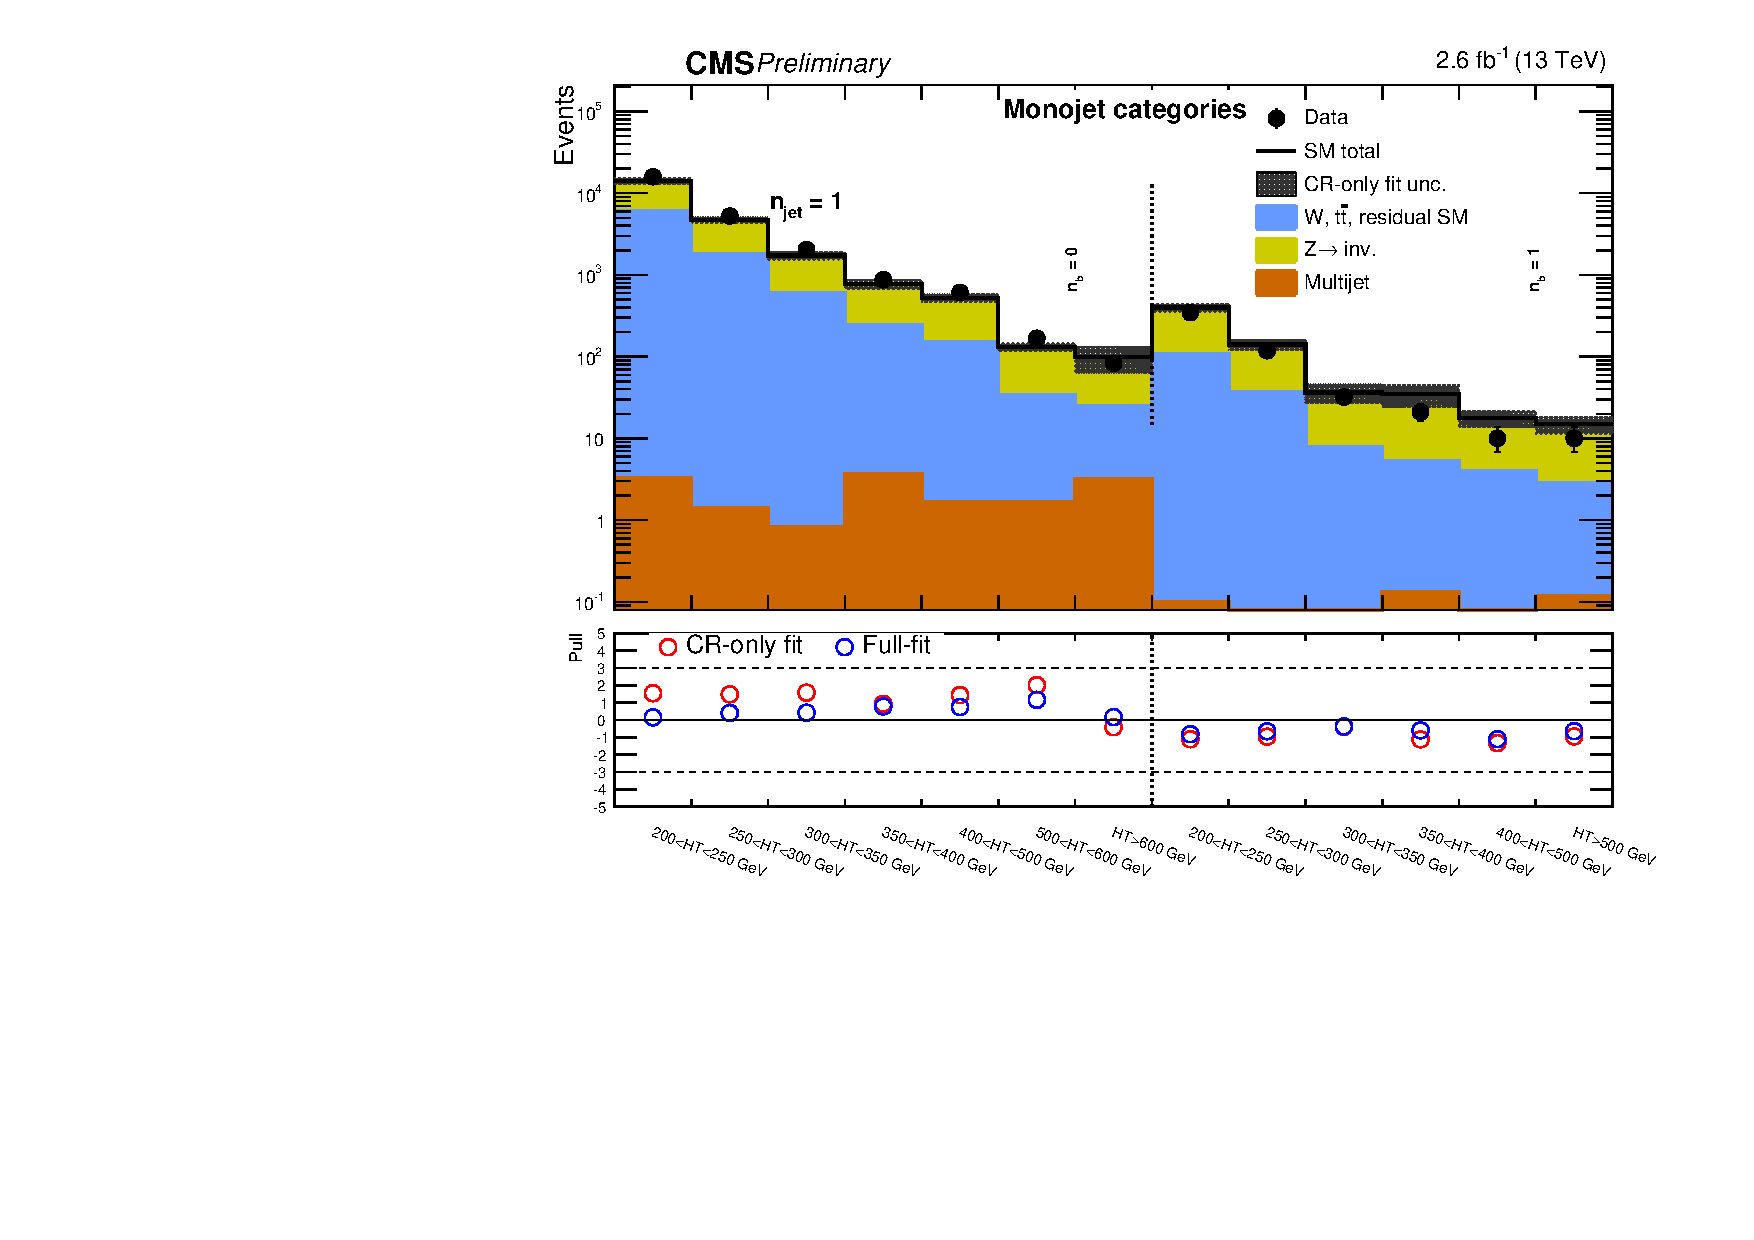
\includegraphics[width=0.7\textwidth]{summaryPlot_Monojet_prefit_overlay_fit_b_CRFit}
    \caption{(Top panel) Event yields observed in data (solid circles)
      and SM expectations with their associated uncertainties (black
      histogram with shaded band) from a CR-only fit, integrated over
      \HTmiss, as a function of \nb, and \scalht for the monojet
      category ($\njet = 1$) in the signal region. (Bottom panel). The
      significance of deviations observed in data with respect to the
      SM expectations from the CR-only (red circles) and full fit
      (blue circles).  }
    \label{fig:mono}
  \end{center}
\end{figure}

\begin{figure*}[!h]
  \begin{center}
    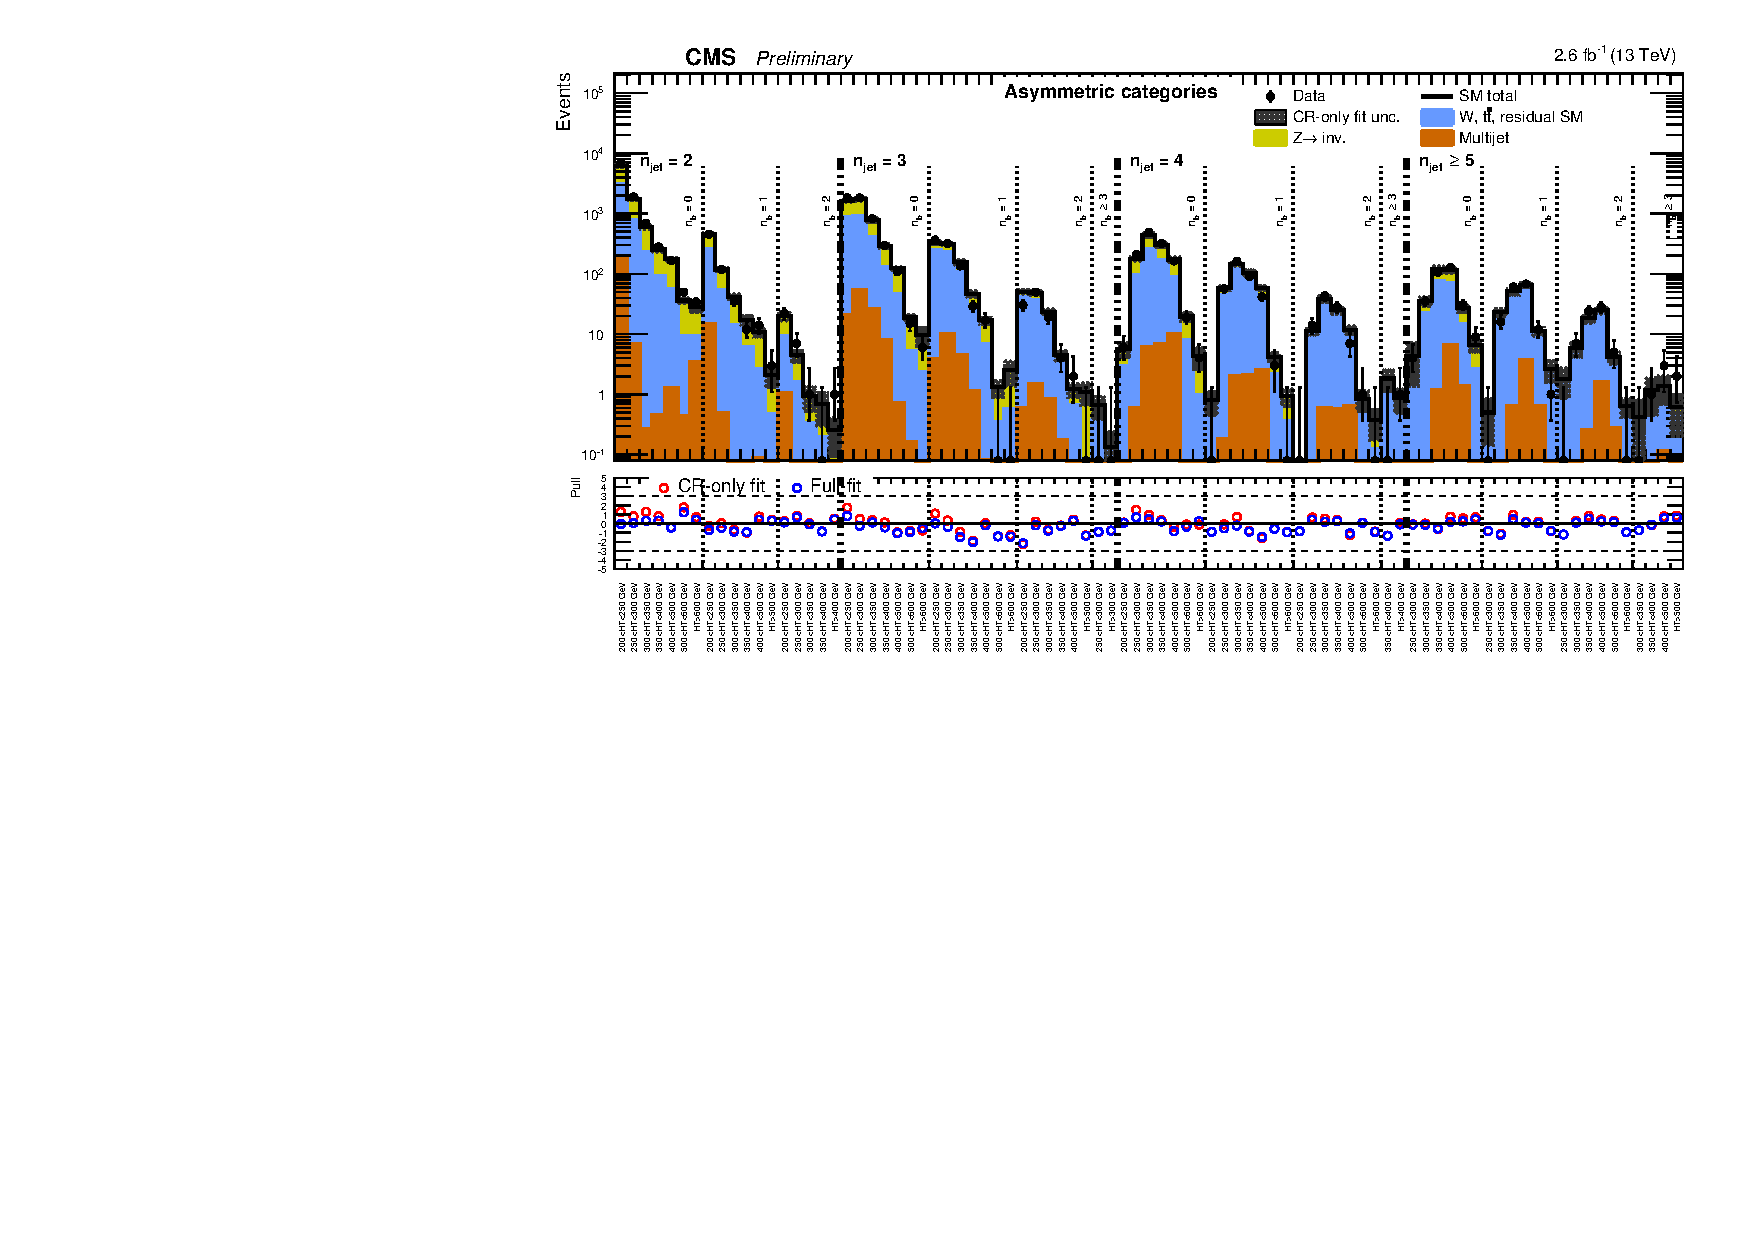
\includegraphics[angle=90,width=0.7\textwidth]{summaryPlot_Asymmetric_prefit_overlay_fit_b_CRFit}
    \caption{(Top panel) Event yields observed in data (solid circles)
      and SM expectations with their associated uncertainties (black
      histogram with shaded band) from a CR-only fit, integrated
      over \HTmiss, as a function of \njet, \nb, and \scalht for the
      ``asymmetric'' \njet categories in the signal region. (Bottom
      panel). The significance of deviations observed in data with
      respect to the SM expectations from the CR-only (red circles)
      and full fit (blue circles).  }
    \label{fig:asym}
  \end{center}
\end{figure*}

\begin{figure*}[!h]
  \begin{center}
    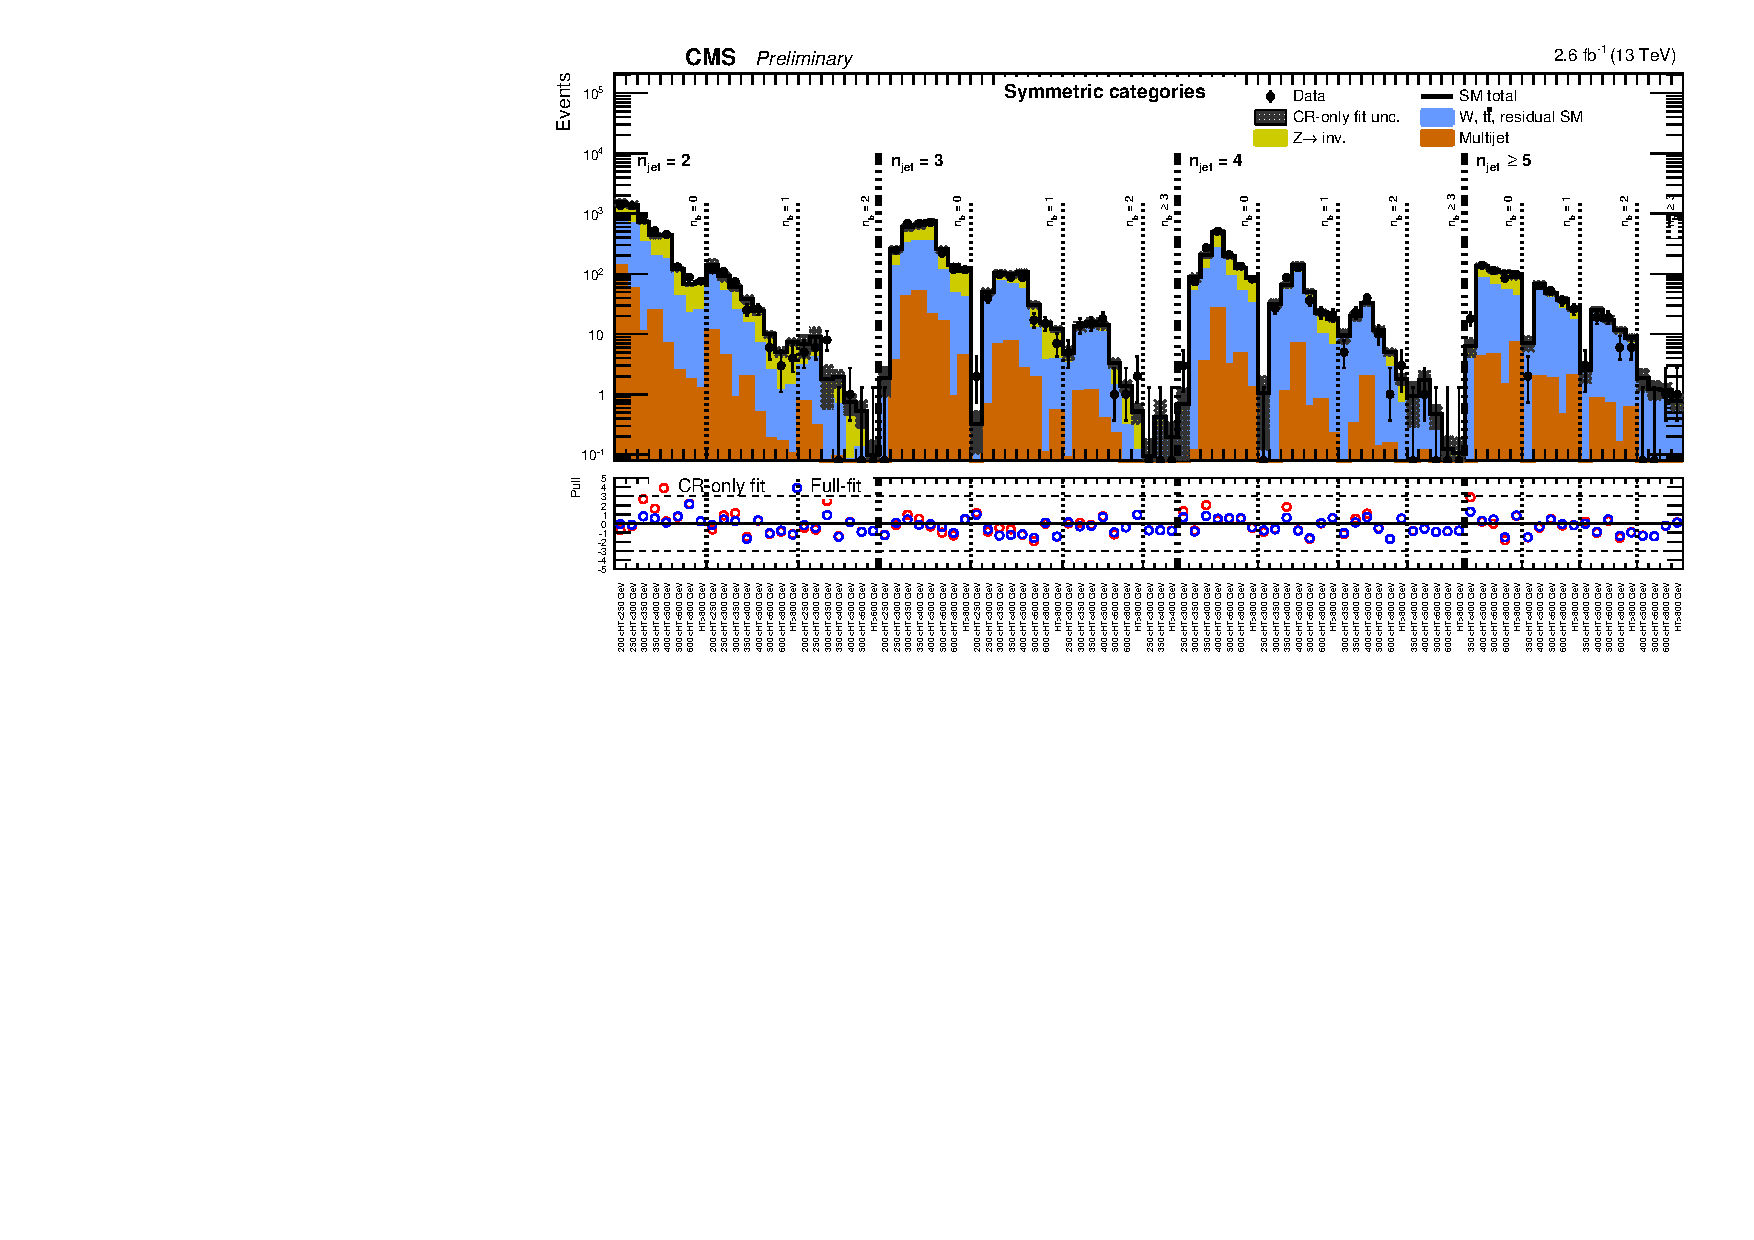
\includegraphics[angle=90,width=0.7\textwidth]{summaryPlot_Symmetric_prefit_overlay_fit_b_CRFit}
    \caption{(Top panel) Event yields observed in data (solid circles)
      and SM expectations with their associated uncertainties (black
      histogram with shaded band) from a CR-only fit, integrated over
      \HTmiss, as a function of \njet, \nb, and \scalht for the
      ``symmetric'' \njet categories in the signal region. (Bottom
      panel). The significance of deviations observed in data with
      respect to the SM expectations from the CR-only (red circles)
      and full fit (blue circles).  }
    \label{fig:sym}
  \end{center}
\end{figure*}

\begin{figure*}[tbhp]
  \begin{center}
    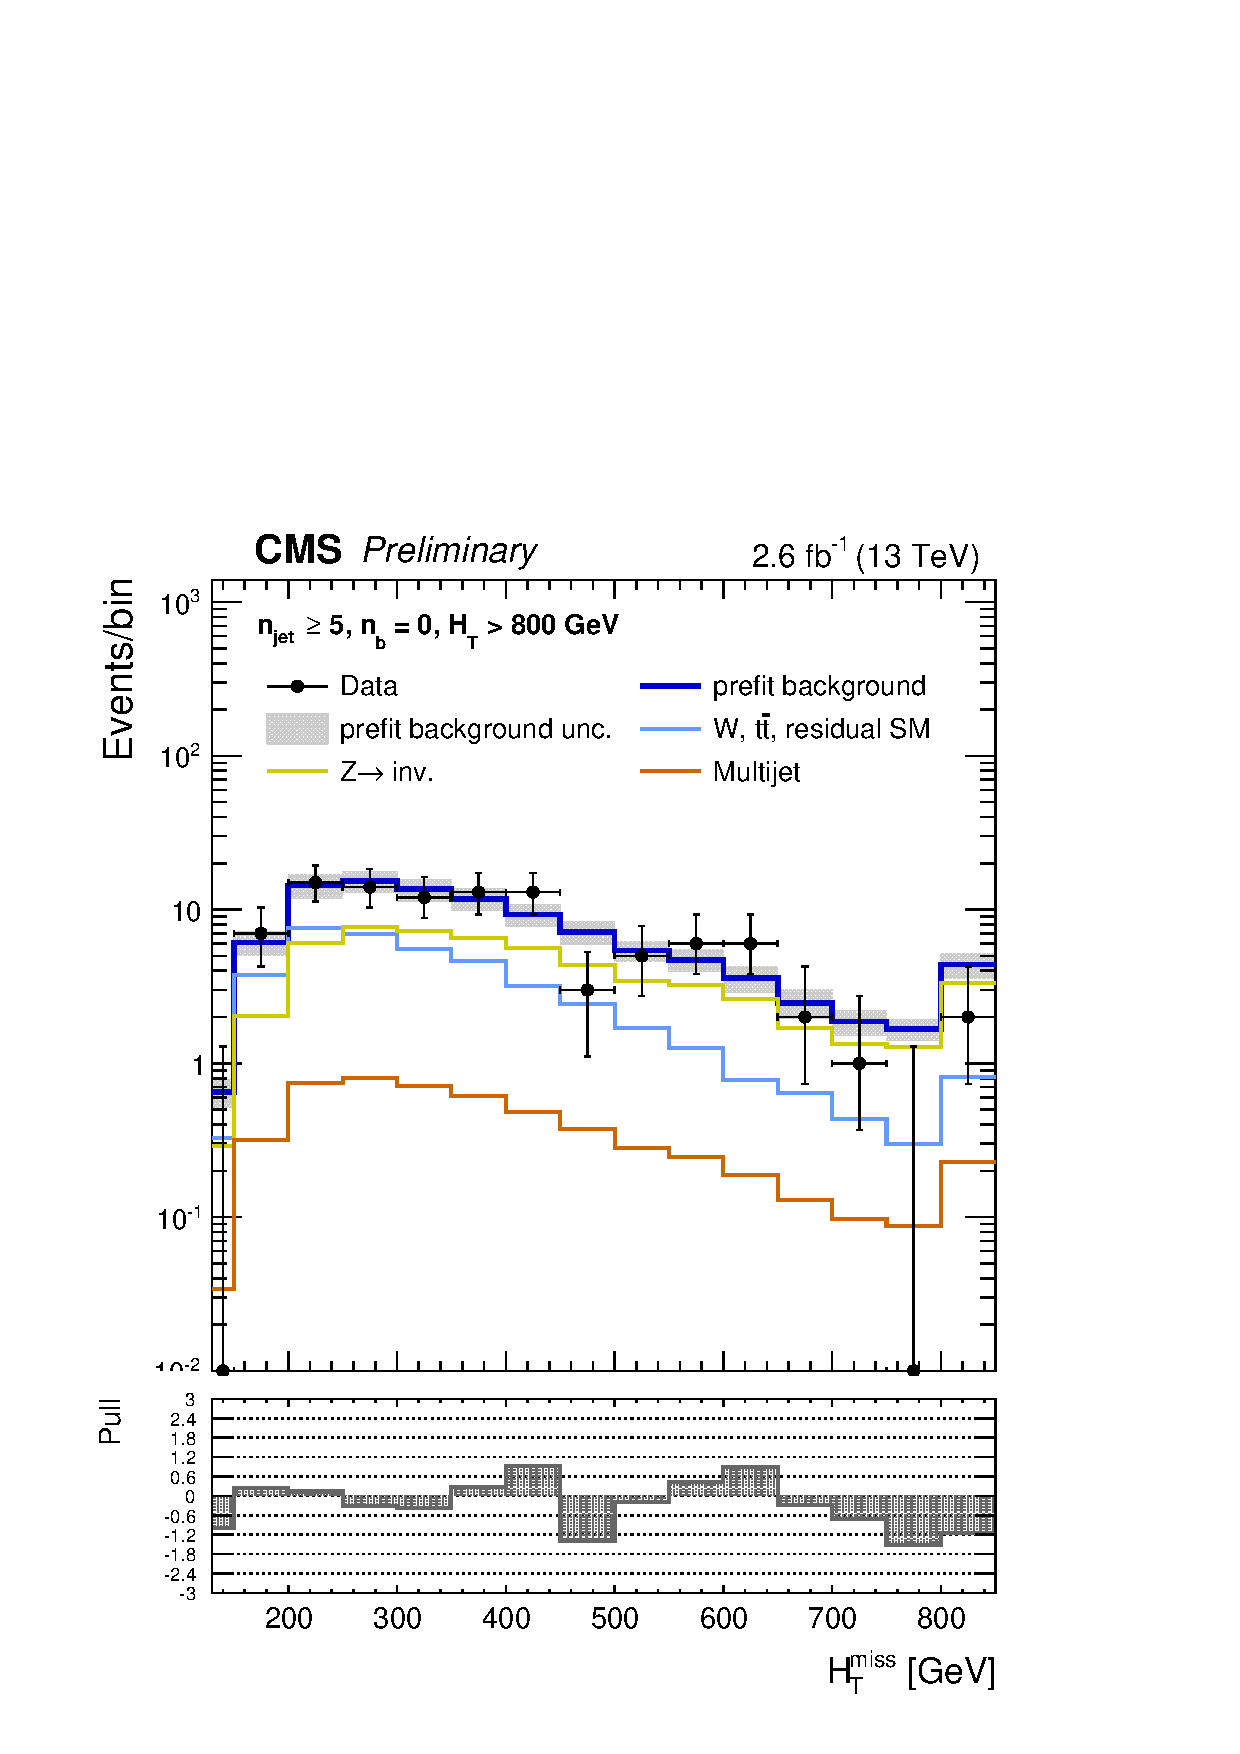
\includegraphics[width=0.6\textwidth]{mhtShape_eq0b_ge5j_800_Inf_prefit.pdf} 
    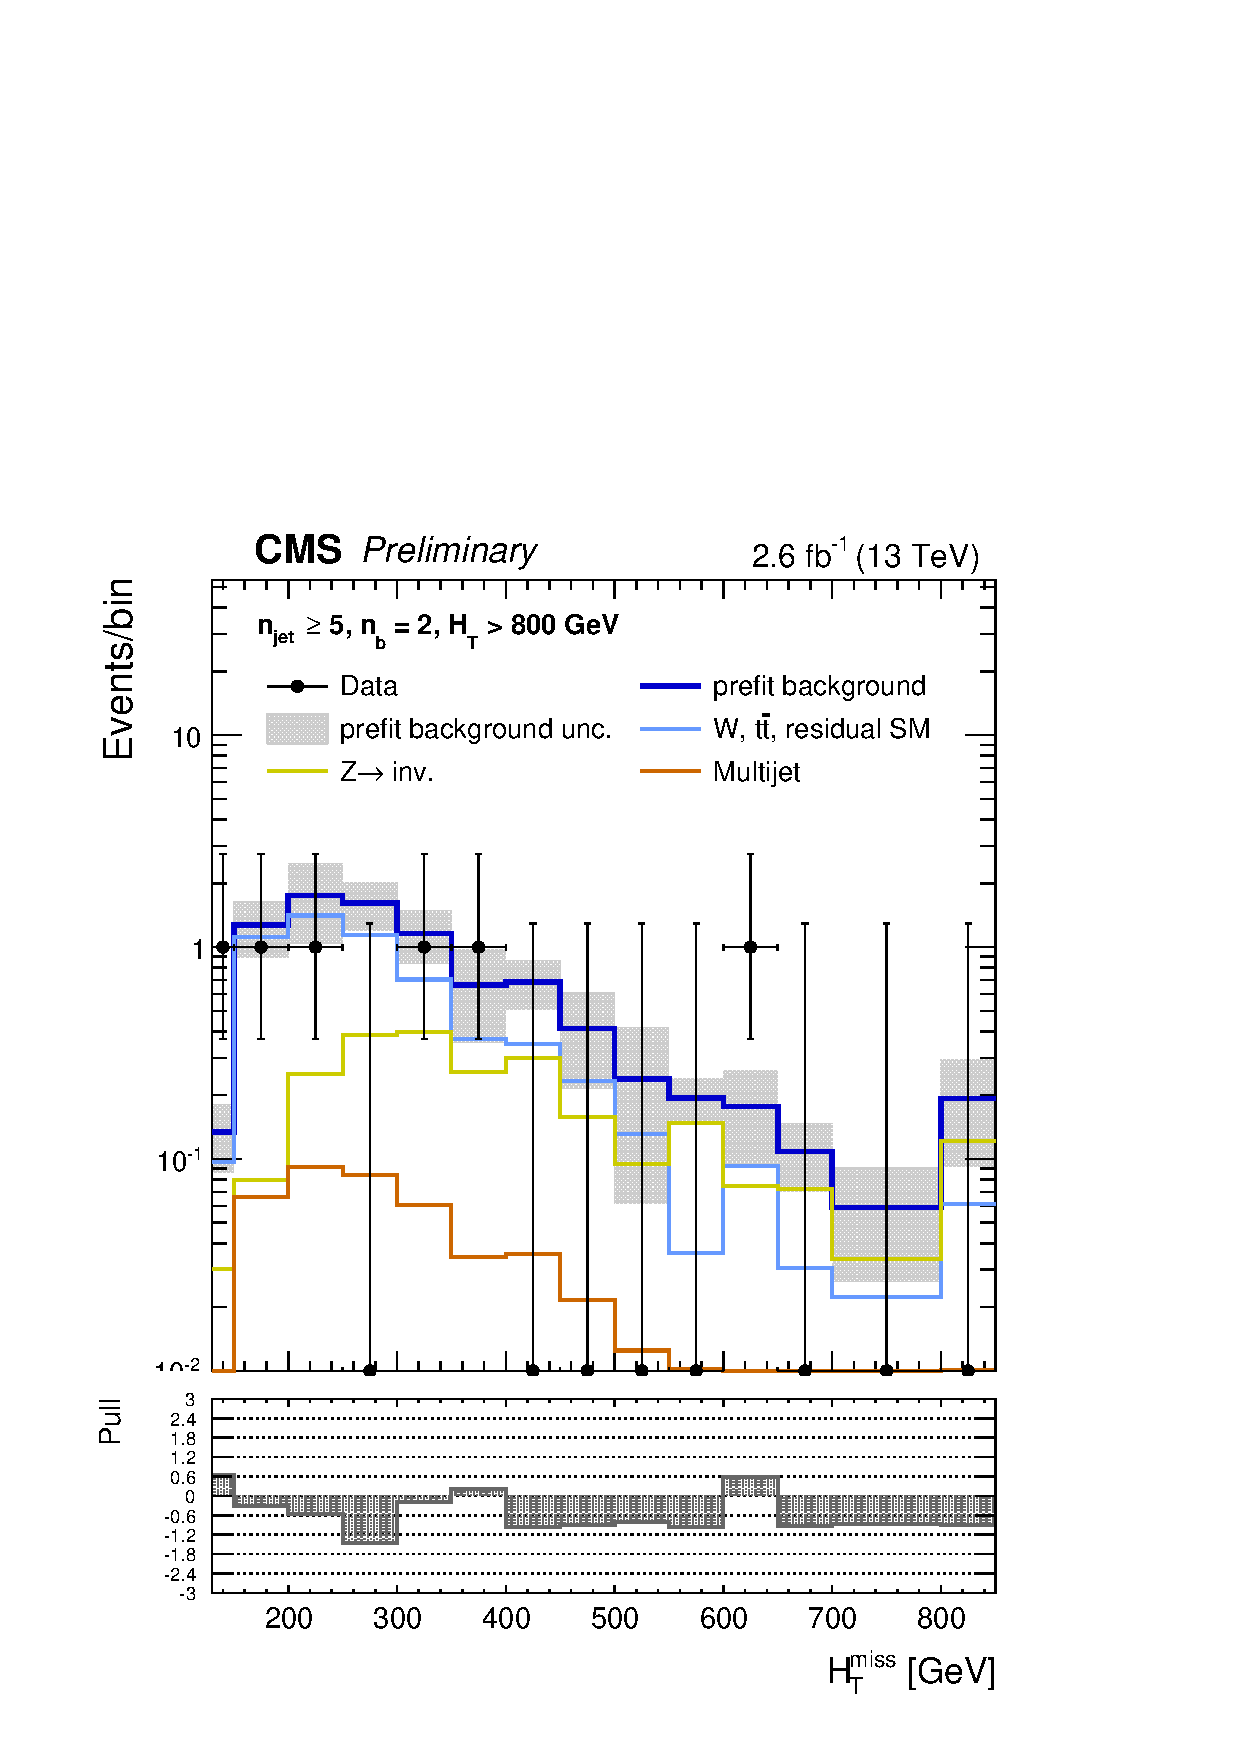
\includegraphics[width=0.6\textwidth]{mhtShape_eq2b_ge5j_800_Inf_prefit.pdf} \\
  \end{center}
  \caption{ The \mht distribution observed in data and the expected
    distribution for the sum of all SM background processes in two
    representative event categories at high \njet and \scalht. 
    \label{fig:mht-templates} }
\end{figure*}

%%__________________________________________________________________||
\clearpage
\section{Interpretation}

The results of this search are interpreted in the context of several simplified models of dark matter as upper limits at a 95\% CL on the ratio of the signal cross section to the predicted cross section as a function of the mediator mass and and WIMP mass. The event samples for the simplified models are generated with \POWHEG V2 using the NNPDF30 PDFs. Various uncertainties in the experimental
acceptance are considered, for which typical magnitudes are summarised in Table~\ref{tab:signal_systs}.

\begin{table}[h!]
  \caption{%CMS {\it Simulation}. 
    Representative magnitudes of systematic uncertainties in the experimental
    acceptance for axial-vector mediated signal models.
  }
  \label{tab:signal_systs}
  \centering
%  \small
  \begin{tabular}{ lccc }
    \hline
    \hline
    Systematic source                   & Type          & Correlated & Typical magnitude (\%) \\
    \hline
    Luminosity                          & Normalisation & Yes        & 6.2                    \\
    Monte Carlo statistics              & Norm. + shape & No         & 1--50                  \\
    Jet energy scale                    & Norm. + shape & Yes        & 1--6                   \\
    b-tag efficiency scale factors      & Norm. + shape & Yes        & 0.4--0.8               \\
    Pile-up                             & Norm. + shape & Yes        & 0-2                    \\
    Trigger efficiency                  & Norm. + shape & Yes        & 0.0--0.3               \\
    Parton distribution functions       & Norm. + shape & Yes        & 1-3                    \\
    Factorisation/renormalisation scale & Norm. + shape & Yes        & 5-9                    \\
    \hline
    \hline
  \end{tabular}
\end{table}
  
%\begin{figure*}[thp!]
%  \begin{center}
%    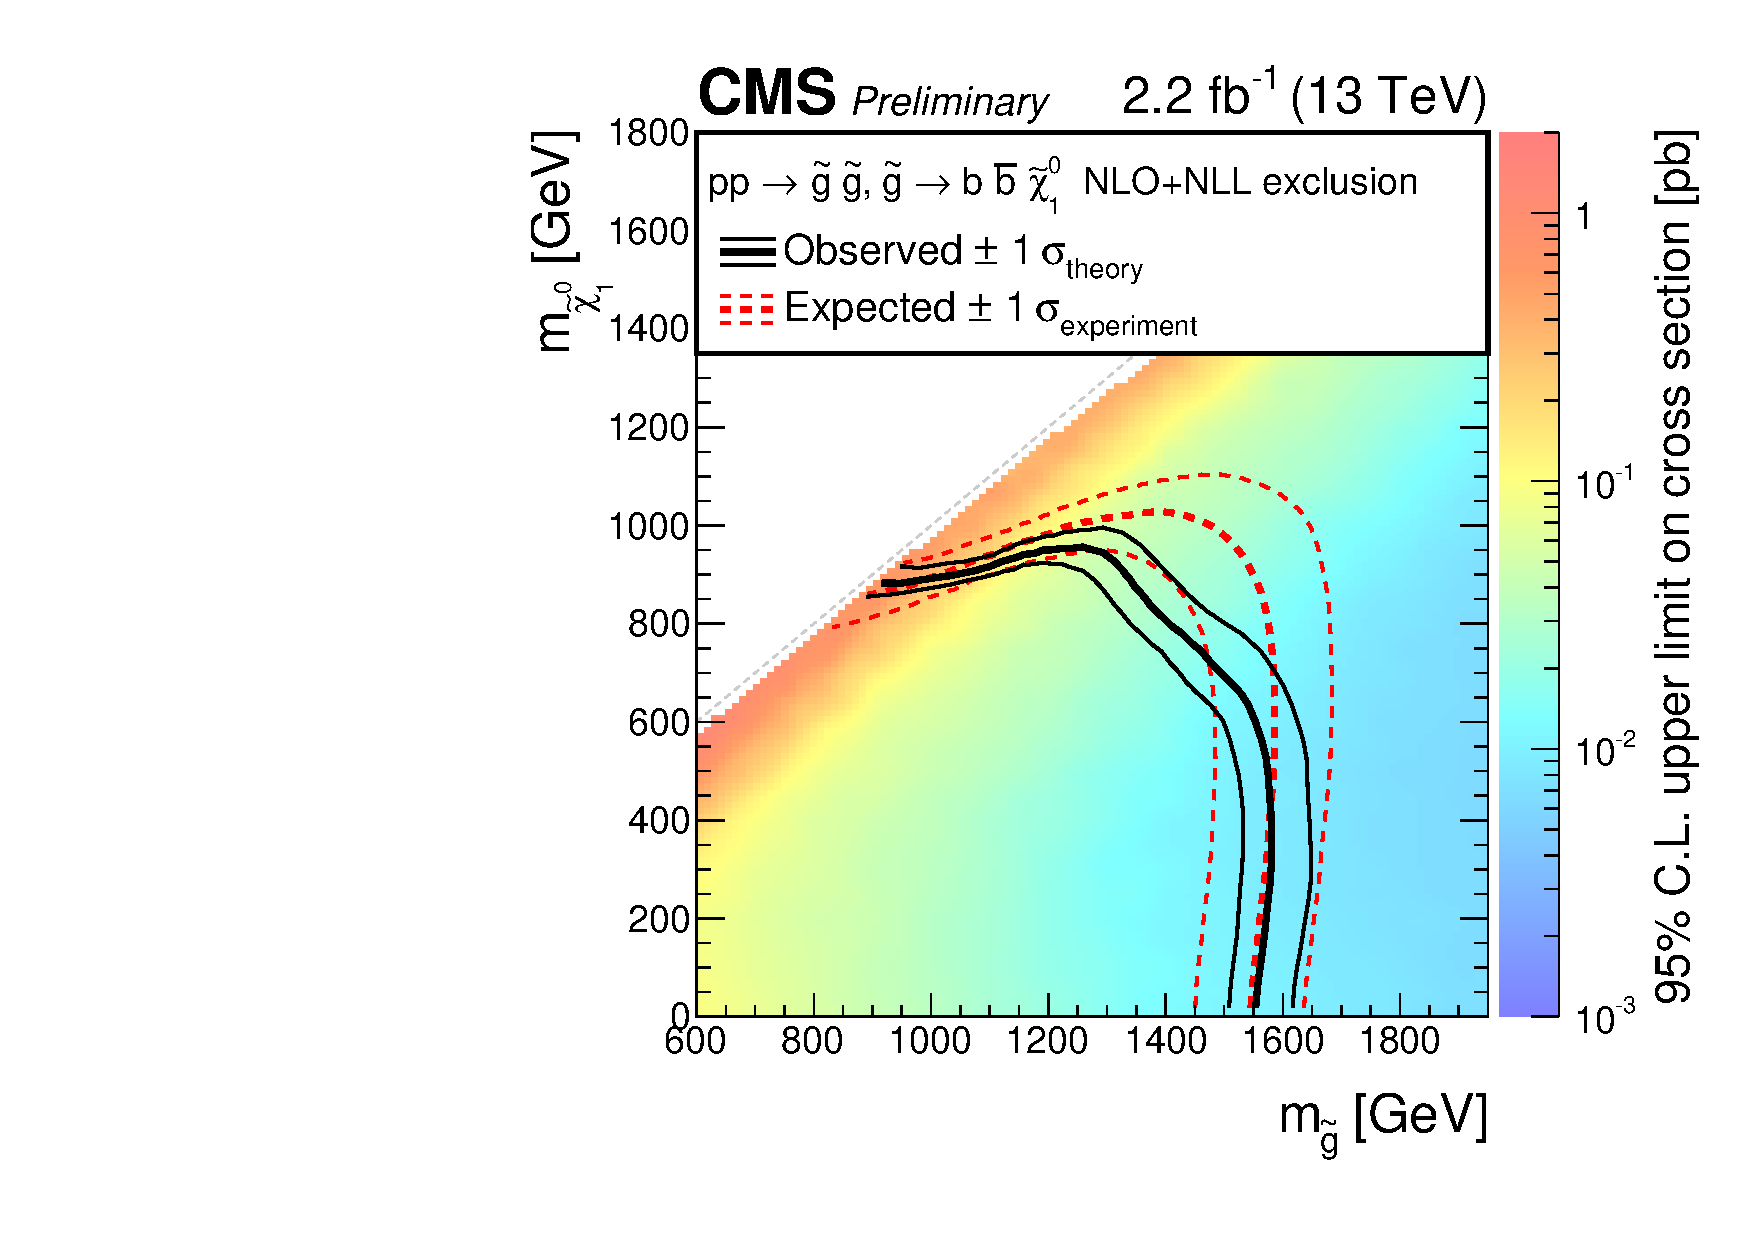
\includegraphics[width=0.49\textwidth]{t1bbbbRA1XSEC.pdf} \,
%    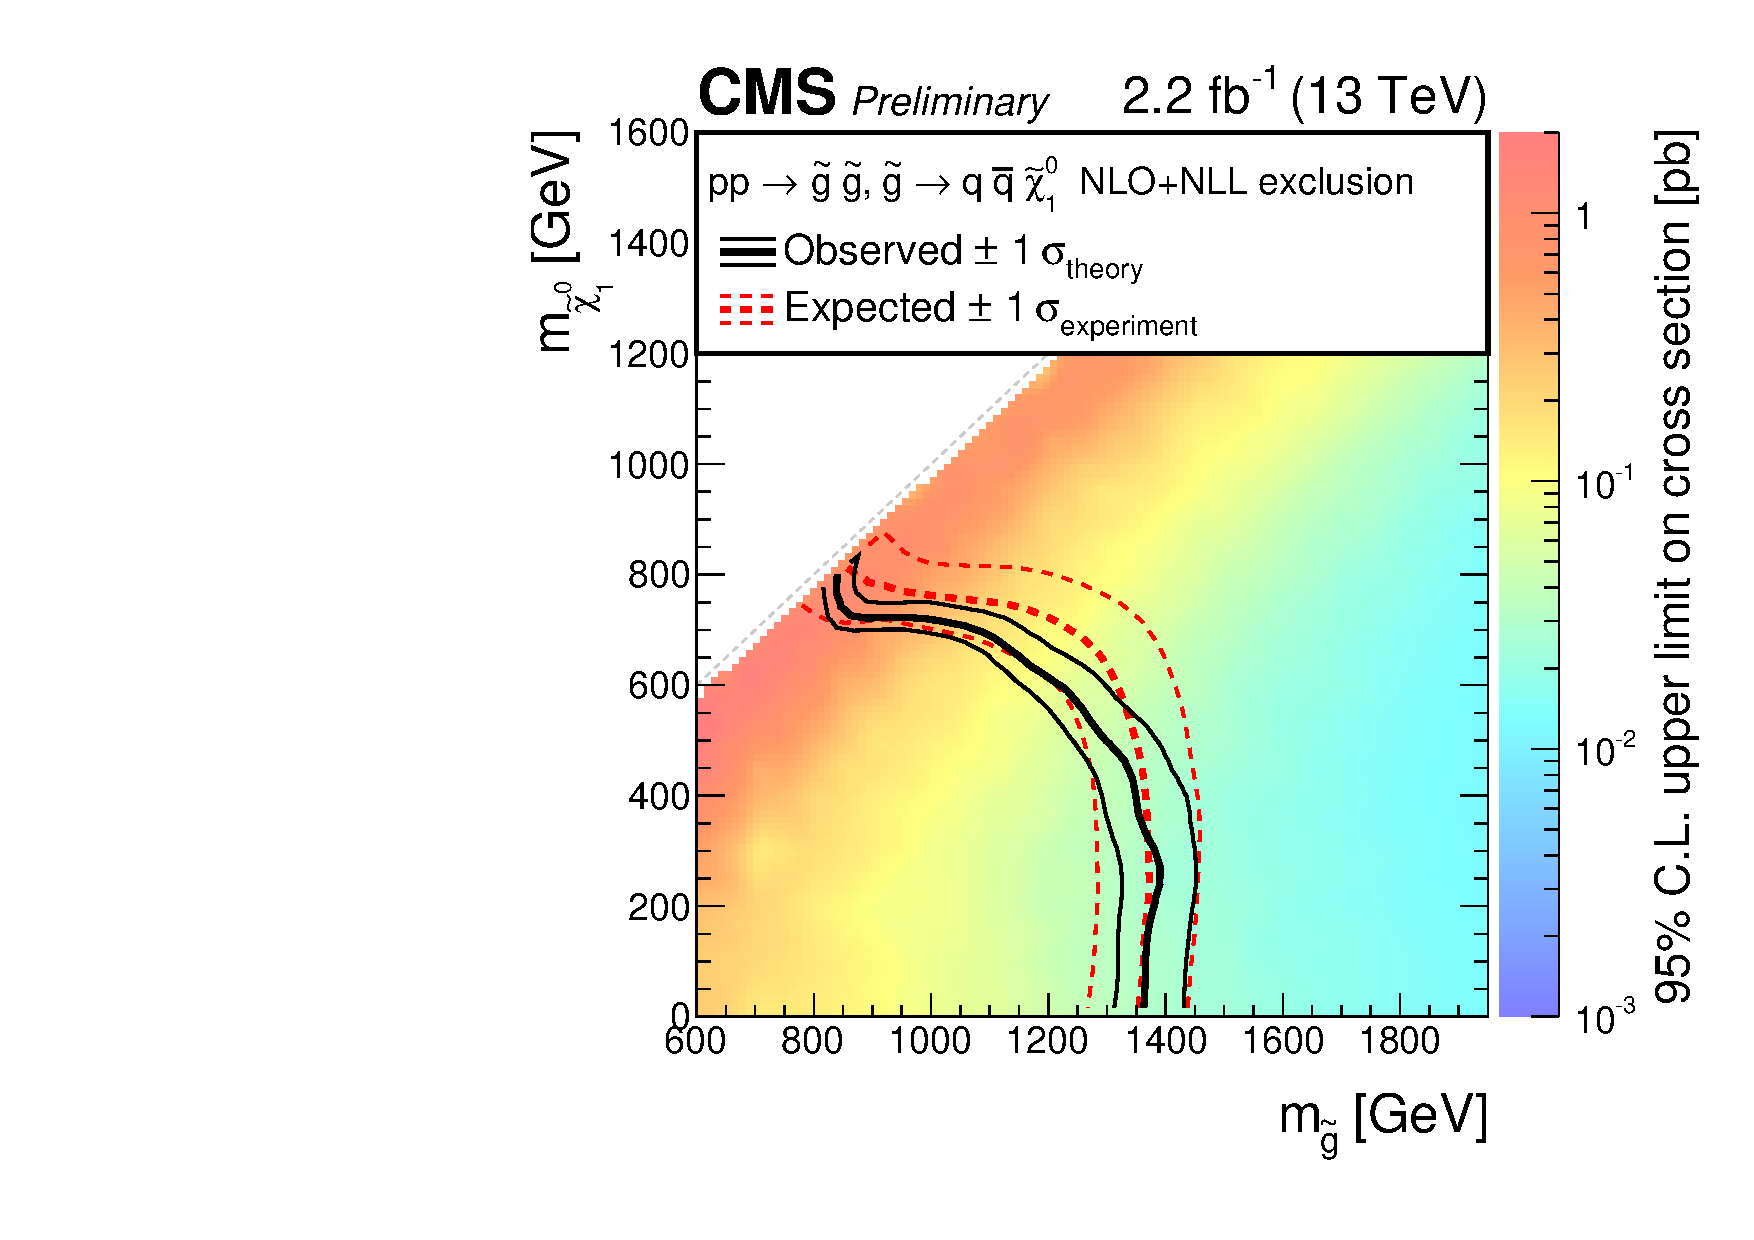
\includegraphics[width=0.49\textwidth]{t1qqqqRA1XSEC.pdf} \\
%    \caption{Observed upper limit in cross section at 95\% CL
%      (indicated by the colour scale) for simplified models that
%      assume the pair production of gluinos, as a function of the
%      gluino and $\chiz_{1}$ masses for gluino three-body decays to
%      $b\bar{b}\chiz_{1}$ (left) and $q\bar{q}\chiz_{1}$ (right). The
%      black solid thick (thin) line indicates the observed mass
%      exclusion region assuming the nominal (${\pm}1 \sigma$ theory
%      uncertainty) production cross section. The red dashed thick
%      (thin) line indicates the median (${\pm}1 \sigma$ experimental
%      uncertainty) expected exclusion.
%      \label{fig:limits-sms} }
%  \end{center}
%\end{figure*}

%Figure~X \fixme{\it will show} 
%\ref{fig:limits-sms} shows 
Tab.~\ref{tab:DMV_limits}-\ref{tab:DMttPS_limits} shows
the expected and observed upper limit on the
%production cross section at 95\% confidence level (CL) as a function
%of the mediator and WIMP masses for a range of simplified models assuming
production cross section at 95\% confidence level (CL) for a range of simplified models assuming
pair production of WIMPs in association with jets originating from light flavour and heavy flavour quarks. The couplings of the mediator to SM particles is assumed to be 0.25 for the axial vector and vector models and 1.0 for the scalar and pseudoscalar models. The couplings of the mediator to WIMPs is assumed to be 1.0 for all models. 
%Upper limits at 95\% CL are also presented on the cross section times branching fraction of the production via gluon fusion of the 125 GeV Higgs boson decaying to a pair of invisible particles. 

%Table shows the expected 95\%CL limits for some signal points for a range of simplified models. 
\begin{table}[h!]
    \caption{%CMS {\it Simulation}.
    95\% CL limits for signal point of the light flavour simplified model 
    mediated by a vector boson. }
    \label{tab:DMV_limits}
    \centering
%    \footnotesize
    \begin{tabular}{ ccc }
        \hline\hline
        M$_{med}$,M$_{DM}$ & r-value (expected) & r-value (observed) \\ 
        \hline
        500, 200  & $0.088_{-0.025}^{+0.036}$ & 0.120 \\
        300, 150  & $0.233_{-0.066}^{+0.094}$ & 0.445 \\
        1000, 350 & $0.323_{-0.091}^{+0.133}$ & 0.239 \\
        1250, 150 & $0.56_{-0.16}^{+0.23}$    & 0.32  \\
        1250, 1   & $0.56_{-0.16}^{+0.23}$    & 0.40  \\
        1250, 350 & $0.57_{-0.16}^{+0.24}$    & 0.40  \\
        1250, 250 & $0.57_{-0.16}^{+0.24}$    & 0.41  \\
        1250, 400 & $0.62_{-0.17}^{+0.25}$    & 0.43  \\
        1500, 200 & $0.96_{-0.27}^{+0.39}$    & 0.73  \\
        1500, 50  & $1.00_{-0.28}^{+0.42}$    & 0.72  \\
        1500, 150 & $1.01_{-0.29}^{+0.42}$    & 0.66  \\
        1500, 100 & $1.03_{-0.29}^{+0.43}$    & 0.66  \\
        \hline\hline
    \end{tabular}
\end{table}

\begin{table}[h!]
    \caption{%CMS {\it Simulation}.
    95\% CL limits for signal point of the light flavour simplified model 
    mediated by an axial-vector boson. }
    \label{tab:DMAV_limits}
    \centering
%    \footnotesize
    \begin{tabular}{ ccc }
        \hline\hline
        M$_{med}$,M$_{DM}$ & r-value (expected) & r-value (observed) \\ 
        \hline
         300, 1    & $0.038_{-0.011}^{+0.015}$ & 0.085 \\
         300, 100  & $0.062_{-0.017}^{+0.026}$ & 0.137 \\
         500, 1    & $0.071_{-0.020}^{+0.028}$ & 0.074 \\
         500, 150  & $0.112_{-0.031}^{+0.046}$ & 0.143 \\
         500, 200  & $0.198_{-0.056}^{+0.081}$ & 0.258 \\
         1000, 300 & $0.46_{-0.13}^{+0.19}$    & 0.33  \\
         1250, 10  & $0.54_{-0.15}^{+0.23}$    & 0.34  \\
         1250, 100 & $0.56_{-0.16}^{+0.23}$    & 0.38  \\
         1000, 350 & $0.58_{-0.16}^{+0.24}$    & 0.57  \\
         1250, 150 & $0.58_{-0.16}^{+0.24}$    & 0.41  \\
         1250, 200 & $0.60_{-0.17}^{+0.25}$    & 0.41  \\
         1250, 250 & $0.64_{-0.18}^{+0.27}$    & 0.51  \\
         1250, 300 & $0.71_{-0.20}^{+0.30}$    & 0.49  \\
         1250, 350 & $0.79_{-0.22}^{+0.32}$    & 0.53  \\
         1500, 150 & $0.99_{-0.28}^{+0.42}$    & 0.58  \\
         1500, 50  & $1.00_{-0.28}^{+0.41}$    & 0.61  \\
         1500, 100 & $1.03_{-0.29}^{+0.43}$    & 0.66  \\
         1500, 200 & $1.08_{-0.31}^{+0.45}$    & 0.69  \\
         1500, 250 & $1.12_{-0.32}^{+0.47}$    & 0.78  \\
         1500, 300 & $1.16_{-0.33}^{+0.48}$    & 0.74  \\
         1500, 350 & $1.23_{-0.35}^{+0.52}$    & 0.77  \\
         1500, 400 & $1.35_{-0.39}^{+0.56}$    & 0.82  \\
        \hline\hline
    \end{tabular}
\end{table}

\begin{table}[h!]
    \caption{%CMS {\it Simulation}.
    95\% CL limits for signal point of the heavy flavour simplified model 
    mediated by a scalar boson. }
    \label{tab:DMttS_limits}
    \centering
%    \footnotesize
    \begin{tabular}{ ccc }
        \hline\hline
        M$_{med}$,M$_{DM}$ & r-value (expected) & r-value (observed) \\ 
        \hline
        10, 1   & $0.63_{-0.20}^{+0.34}$ & 0.43 \\
        20, 1   & $0.76_{-0.24}^{+0.41}$ & 0.37 \\
        50, 10  & $1.00_{-0.32}^{+0.55}$ & 0.59 \\
        50, 1   & $1.14_{-0.36}^{+0.62}$ & 0.73 \\
        100, 1  & $1.52_{-0.49}^{+0.83}$ & 1.10 \\
        100, 10 & $1.59_{-0.51}^{+0.88}$ & 1.35 \\
        200, 50 & $2.84_{-0.93}^{+1.59}$ & 3.81 \\
        200, 1  & $2.84_{-0.93}^{+1.59}$ & 3.46 \\
        300, 50 & $4.5_{-1.5}^{+2.6}$    & 4.8  \\
        300, 1  & $4.6_{-1.5}^{+2.7}$    & 6.8  \\
        500, 1  & $16.4_{-5.6}^{+10.1}$  & 22.0 \\
        15, 10  & $24.1_{-7.8}^{+13.1}$  & 14.1 \\
        10, 10  & $27.1_{-8.8}^{+14.4}$  & 25.8 \\
        95, 50  & $68_{-22}^{+39}$       & 77   \\
        50, 50  & $123_{-41}^{+71}$      & 142  \\
        10, 50  & $138_{-46}^{+80}$      & 150  \\
        \hline\hline
    \end{tabular}
\end{table}

\begin{table}[h!]
    \caption{%CMS {\it Simulation}.
    95\% CL limits for signal point of the heavy flavour simplified model 
    mediated by a pseudoscalar boson. }
    \label{tab:DMttPS_limits}
    \centering
%    \footnotesize
    \begin{tabular}{ ccc }
        \hline\hline
        M$_{med}$,M$_{DM}$ & r-value (expected) & r-value (observed) \\ 
        \hline
        10, 1   & $1.32_{-0.44}^{+0.77}$ & 1.40 \\
        20, 1   & $1.33_{-0.44}^{+0.77}$ & 1.35 \\
        50, 10  & $1.38_{-0.46}^{+0.81}$ & 1.74 \\
        50, 1   & $1.45_{-0.48}^{+0.84}$ & 1.50 \\
        100, 10 & $1.60_{-0.54}^{+0.93}$ & 2.34 \\
        100, 1  & $1.60_{-0.53}^{+0.94}$ & 2.11 \\
        200, 50 & $2.34_{-0.79}^{+1.40}$ & 3.08 \\
        200, 1  & $2.35_{-0.80}^{+1.41}$ & 3.22 \\
        300, 50 & $3.6_{-1.2}^{+2.2}$    & 5.5  \\
        300, 1  & $3.6_{-1.2}^{+2.2}$    & 4.9  \\
        500, 1  & $17.4_{-6.2}^{+11.0}$  & 23.3 \\
        15, 10  & $20.3_{-6.7}^{+12.0}$  & 25.9 \\
        95, 50  & $23.7_{-8.0}^{+14.0}$  & 27.7 \\
        10, 10  & $24.0_{-8.1}^{+14.1}$  & 22.7 \\
        50, 50  & $66_{-22}^{+40}$       & 93   \\
        10, 50  & $78_{-26}^{+48}$       & 131  \\
        \hline\hline
    \end{tabular}
\end{table}

\clearpage

%%__________________________________________________________________||
